\documentclass[12pt,fleqn]{article}\usepackage{../../common}
\begin{document}
Sayısal Kontrol ve Sınır Değer Problemleri (BVP)

Bu bölümde optimal kontrol problemlerini sayısal çözmenin yöntemlerini
göreceğiz. 

Rayleigh Problemi

Bir elektrik devresi düşünelim, bu devre düz voltajı salınıma çevirebiliyor, 

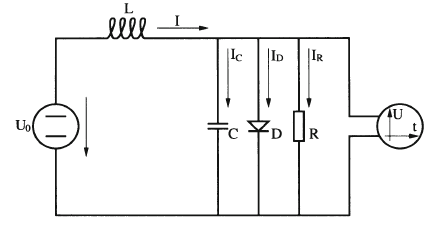
\includegraphics[width=20em]{phy_num_01.png}

Devreyi sol taraftan verilen $U_0(t)$ ile kontrol etmek mümkün [1,
sf. 189], [2, sf. 413]. Devreninin denklemi

$$
\ddot{x} = -x(t) + \dot{x}(t) ( 2.0 - p \dot{x}(t)^2 ) +  u(t)
$$

ki biz $p = 0.1$ seçeceğiz, ve konum değişkeni $x(t)$ $t$ anındaki elektrik
akımı $I$'yı temsil ediyor. ODE sistemini çıkartmak için $x_1 = x$,
$x_2 = \dot{x}$ dersek,

$$
\dot{x_2} = -x_1 + (2.0 - 0.1 x_2^2)x_2 + 4 u(t)
$$

Acaba $x_1(t=0)=-5$ ve $x_2(t=0)=-5$ başlangıç şartları için,
$t_f=2.5$ anına kadar kontrolü ve salınımı az seviyede tutmaya
çalışsak nasıl bir kontrol uygulamamız gerekir?

Yani minimize etmek istedigimiz, 

$$
J(u) = \int_{0}^{2.5} V  \ud t = \int_{0}^{2.5} (x_1^2 + u^2)  \ud t
$$

ki $V = x_1^2 + u^2$.

Not: Üstteki formül tam formül $J(u) = \phi(x(t_f) + \int_{0}^{2.5} V  \ud
t$ formulunden biraz farklı, $\phi$ yok, yani varılan son konum için bir
bedel tanımlanmadı. Bunun sonucu $\lambda(t_f)$'in sıfır olmasıdır.

Hamiltonian'ı tanımlarken

$$
\mathcal{H} = V + \lambda^T f
$$

formülü verilmişti. $f$ formülü üstte görülen $\dot{x}_1$ ve
$\dot{x}_2$'den oluşuyor tabii.

Şimdi $\mathcal{H}$'yi sembolik olarak bulalım,

\begin{minted}[fontsize=\footnotesize]{python}
import sympy

u, x1, x2, lam1, lam2 = sympy.symbols('u x1 x2 lam1 lam2')
x = sympy.Matrix([[x1],[x2]])
lam = sympy.Matrix([[lam1],[lam2]])
f = sympy.Matrix([[x[1]],[  -x[0]+(2.0 - 0.1*x[1]**2)*x[1] + 4*u ]])
V = x[0]**2 + u**2
H = V + lam.T.dot(f)
print (H)
print (sympy.latex(H))
\end{minted}

\begin{verbatim}
lam1*x2 + lam2*(4*u - x1 + x2*(2.0 - 0.1*x2**2)) + u**2 + x1**2
lam_{1} x_{2} + lam_{2} \left(4 u - x_{1} + x_{2} \left(2.0 - 0.1 x_{2}^{2}\right)\right) + u^{2} + x_{1}^{2}
\end{verbatim}


$$
\mathcal{H} = \lambda_{1} x_{2} + \lambda_{2} \left(4 u - x_{1} + x_{2} \left(2.0 - 0.1
x_{2}^{2}\right)\right) + u^{2} + x_{1}^{2}
$$

Eğer bu formülü biraz masajlarsak, [2]'deki sonucu elde ederiz,

$$
= x_1^2 + u^2 + \lambda_1 x_2 - \lambda_2
\left( x_1 - 4u + x_2 \left( \frac{x_2^2}{10} - 2 \right)  \right)
$$

$\dot{\lambda} = -(\partial \mathcal{H} / \partial x)^T$ ve  $\lambda(t_f) = (\partial \phi / \partial x)^T$ üzerinden ,

\begin{minted}[fontsize=\footnotesize]{python}
lam_dot = -sympy.diff(H, x).T
print (lam_dot)
\end{minted}

\begin{verbatim}
Matrix([[lam2 - 2*x1, -lam1 - lam2*(2.0 - 0.3*x2**2)]])
\end{verbatim}


$$
\left[\begin{array}{c}
\dot{\lambda_1} \\ \dot{\lambda_2} 
\end{array}\right] =
\left[\begin{array}{c}
\lambda_2 - 2 x_1 \\
\lambda_1 \left( \frac{3 x_2^2}{10} - 2  \right) - \lambda_1
\end{array}\right],
\quad
\left[\begin{array}{c}
\lambda_1(t_f) \\ \lambda_2(t_f) 
\end{array}\right] =
\left[\begin{array}{c}
0 \\ 0
\end{array}\right]
$$

Optimal kontrol girdisi için $u(t)$'yi için bir çözüm bulmayı gerektiriyor,

\begin{minted}[fontsize=\footnotesize]{python}
u, x1, x2, lam1, lam2 = sympy.symbols('u x1 x2 lam1 lam2')
HH = lam1*x2 + u**2 + x1**2 - lam2*(x1 - 4*u + x2*(x2**2/10 - 2))
uopt = sympy.solve(HH.diff(u),u)[0]
print ( uopt )
\end{minted}

\begin{verbatim}
-2*lam2
\end{verbatim}

Yani

$$
u^*(t) = -2 \lambda_2(t)
$$

sonucuna eriştik. Bulduğumuz optimal $u^*$ değerini $f$ denklemindeki
$u$'lar yerine koyarsak,

\begin{minted}[fontsize=\footnotesize]{python}
x_dot = f.subs({u: uopt})
print (x_dot)
\end{minted}

\begin{verbatim}
Matrix([[x2], [-8*lam2 - x1 + x2*(2.0 - 0.1*x2**2)]])
\end{verbatim}

Daha önceden bulduğumuz $\dot{\lambda}$ formülünü hatırlayalım,

\begin{minted}[fontsize=\footnotesize]{python}
print (lam_dot)
\end{minted}

\begin{verbatim}
Matrix([[lam2 - 2*x1, -lam1 - lam2*(2.0 - 0.3*x2**2)]])
\end{verbatim}

Artık elimizde bir iki noktalı sınır problemi var, bu problemi sayısal
olarak çözebiliriz. 

$$
\left[\begin{array}{c}
\dot{x}_1 \\ 
\dot{x}_2 \\ 
\dot{\lambda}_1 \\ 
\dot{\lambda}_2 
\end{array}\right] = 
\left[\begin{array}{c}
x_2 \\ 
-x_1 + (2 - 0.1 x_2^2 ) x_2 - 8 \lambda_2 \\
\lambda_2 \\
\lambda_1 \left( \frac{3x_2^2}{10} - 2  \right) - \lambda_1
\end{array}\right], 
\quad
\left[\begin{array}{c}
x_1(0) \\ x_2(0) \\ \lambda_1(t_f) \\ \lambda_2(t_f)
\end{array}\right] = 
\left[\begin{array}{c}
-5 \\ -5 \\ 0 \\ 0
\end{array}\right]
$$


\begin{minted}[fontsize=\footnotesize]{python}
from scipy.integrate import solve_bvp

def fun(x, y):
    return np.vstack((
        y[1],
        -8*y[3] - y[0] - y[1]*(y[1]**2/10.0),
        y[3]-2*y[0],
        y[3]*(3/10*y[1]**2-2) - y[2]
        )
    )

def bc(ya, yb):
    return np.array( [ ya[0]+5, ya[1]+5, yb[2], yb[3] ]   )
                     
t = np.linspace(0, 2.5, 10)
y = np.ones((4, t.size))
sol = solve_bvp(fun, bc, t, y)
print (y.shape)
print (sol.y[0].shape)
\end{minted}

\begin{verbatim}
(4, 10)
(35,)
\end{verbatim}

\begin{minted}[fontsize=\footnotesize]{python}
df = pd.DataFrame()
df['x1'] = sol.y[0]
df['x2'] = sol.y[1]
df.plot()
plt.savefig('phy_num_02.png')
\end{minted}

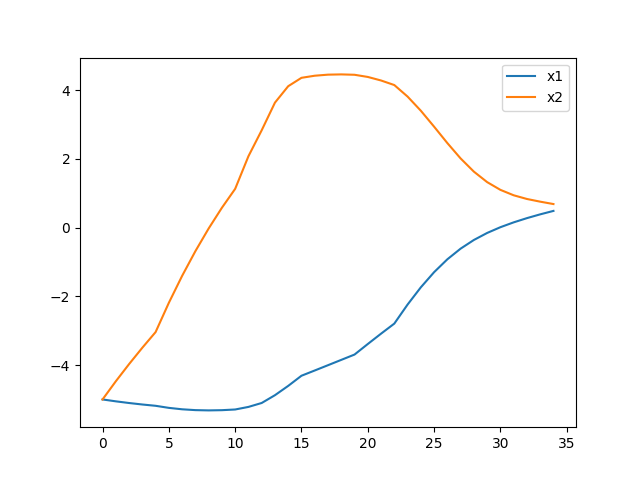
\includegraphics[height=6cm]{phy_num_02.png}

\begin{minted}[fontsize=\footnotesize]{python}
df = pd.DataFrame()
df['$\lambda_1$'] = sol.y[2]
df['$\lambda_2$'] = sol.y[3]
df.plot()
plt.savefig('phy_num_03.png')
\end{minted}

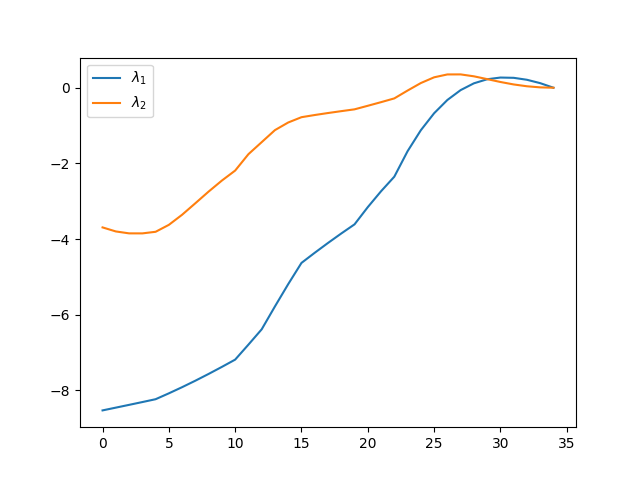
\includegraphics[height=6cm]{phy_num_03.png}

\begin{minted}[fontsize=\footnotesize]{python}
df = pd.DataFrame()
df['u'] = -2*sol.y[3]
df.plot()
plt.savefig('phy_num_04.png')
\end{minted}

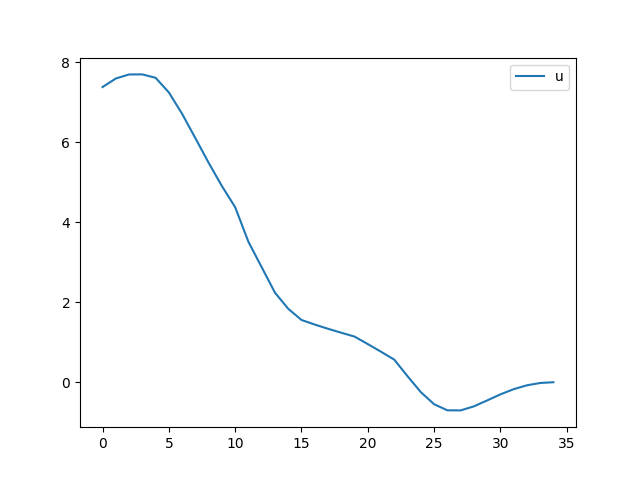
\includegraphics[height=6cm]{phy_num_04.png}

Son grafikte optimal kontrol politikasını görüyoruz. 

Kaynaklar

[1] Bittner, {\em Variational calculus, optimal control and applications}

[2] Wilson, {\em Advanced Control using MATLAB}

\end{document}

